\documentclass[]{article}
\usepackage{lmodern}
\usepackage{amssymb,amsmath}
\usepackage{ifxetex,ifluatex}
\usepackage{fixltx2e} % provides \textsubscript
\ifnum 0\ifxetex 1\fi\ifluatex 1\fi=0 % if pdftex
  \usepackage[T1]{fontenc}
  \usepackage[utf8]{inputenc}
\else % if luatex or xelatex
  \ifxetex
    \usepackage{mathspec}
  \else
    \usepackage{fontspec}
  \fi
  \defaultfontfeatures{Ligatures=TeX,Scale=MatchLowercase}
\fi
% use upquote if available, for straight quotes in verbatim environments
\IfFileExists{upquote.sty}{\usepackage{upquote}}{}
% use microtype if available
\IfFileExists{microtype.sty}{%
\usepackage[]{microtype}
\UseMicrotypeSet[protrusion]{basicmath} % disable protrusion for tt fonts
}{}
\PassOptionsToPackage{hyphens}{url} % url is loaded by hyperref
\usepackage[unicode=true]{hyperref}
\hypersetup{
            pdfborder={0 0 0},
            breaklinks=true}
\urlstyle{same}  % don't use monospace font for urls
\usepackage{graphicx,grffile}
\makeatletter
\def\maxwidth{\ifdim\Gin@nat@width>\linewidth\linewidth\else\Gin@nat@width\fi}
\def\maxheight{\ifdim\Gin@nat@height>\textheight\textheight\else\Gin@nat@height\fi}
\makeatother
% Scale images if necessary, so that they will not overflow the page
% margins by default, and it is still possible to overwrite the defaults
% using explicit options in \includegraphics[width, height, ...]{}
\setkeys{Gin}{width=\maxwidth,height=\maxheight,keepaspectratio}
\IfFileExists{parskip.sty}{%
\usepackage{parskip}
}{% else
\setlength{\parindent}{0pt}
\setlength{\parskip}{6pt plus 2pt minus 1pt}
}
\setlength{\emergencystretch}{3em}  % prevent overfull lines
\providecommand{\tightlist}{%
  \setlength{\itemsep}{0pt}\setlength{\parskip}{0pt}}
\setcounter{secnumdepth}{0}
% Redefines (sub)paragraphs to behave more like sections
\ifx\paragraph\undefined\else
\let\oldparagraph\paragraph
\renewcommand{\paragraph}[1]{\oldparagraph{#1}\mbox{}}
\fi
\ifx\subparagraph\undefined\else
\let\oldsubparagraph\subparagraph
\renewcommand{\subparagraph}[1]{\oldsubparagraph{#1}\mbox{}}
\fi

% set default figure placement to htbp
\makeatletter
\def\fps@figure{htbp}
\makeatother


\date{}

\begin{document}

\section{Kafka: streaming data}\label{kafka-streaming-data}

\subsection{Indice}\label{indice}

\begin{enumerate}
\def\labelenumi{\arabic{enumi}.}
\tightlist
\item
  \protect\hyperlink{motivazioni}{Motivazioni}
\item
  \protect\hyperlink{introduzione}{Introduzione}
\item
  \protect\hyperlink{etl}{ETL}
\item
  \protect\hyperlink{event-sourcing}{Event sourcing}\\
  4.1. \protect\hyperlink{intro-data}{L'importanza dei dati e degli
  eventi}\\
  4.2. \protect\hyperlink{es-desc}{Descrizione}\\
  4.3. \protect\hyperlink{es-vantaggi}{Vantaggi}\\
  4.4. \protect\hyperlink{es-svantaggi}{Svantaggi}
\item
  \protect\hyperlink{kafka-desc}{Apache Kafka: a streaming platform}\\
  5.1. {[}Descrizione ed uso di una streaming platform{]}\\
  5.2. {[}L'architettura di Kafka{]}\\
  5.3. {[}Competitors e soluzioni alternative{]}
\item
  {[}L'ecosistema di Kafka{]}\\
  6.1. {[}Kafka Connect{]}\\
  6.2. {[}Kafka Streams{]}
\item
  {[}Conclusioni{]}
\item
  {[}Esempi di utilizzo{]}
\item
  {[}Bibliografia{]}
\end{enumerate}

\newpage

\hypertarget{motivazioni}{\subsection{1.
Motivazioni}\label{motivazioni}}

Negli ultimi anni l'avvento delle architetture a microservizi ha portato
la necessità di studiare nuove soluzioni al problema della gestione di
molteplici fonti di dati.

In sistemi complessi formati da più microservizi tanti componenti
interdipendenti comunicano tra loro scambiandosi dati e attingendo da
numerose fonti di dati comuni come database, data warehouses oppure
servizi esterni.

La necessità di filtrare, standardizzare e gestire molte fonti di dati
aveva portato alla nascita del processo di \textbf{Extract, Transform,
Load} (ETL) per l'estrazione, trasformazione e caricamento di dati in
sistemi di sintesi come data warehouse o data mart, questo processo si
sta però rivelando complicato ed impegnativo in un mondo dove la mole di
dati prodotta dal logging di eventi critici ad un qualsiasi business è
in continua crescita: semplici esempi sono la gestione degli eventi in
un sistema \textbf{Internet of things} (IoT) oppure lo studio delle
abitudini dei propri clienti per un servizio di e-commerce.

Lo stream processing tra microservizi propone un nuovo approccio per la
gestione di questi problemi, fornendo una soluzione adatta alla gestione
di dati in real-time altamente scalabile e ad alto throughput.

Apache Kafka è una piattaforma di streaming dati nata in un contesto
aziendale importante che mira a rivoluzionare il modo con cui i
microservizi di un business comunicano tra loro, favorendo un approccio
improntato sulla gestione di eventi legati al comportamento dei dati,
più che i dati in se.\\
Kafka nasce per sfruttare a pieno lo stream processing e favorire una
gestione intelligente di grosse moli di dati, abbandonando il classico
processo ``batch'' ETL per una soluzione, appunto, basata sullo
streaming dei dati tra microservizi.

\newpage

\hypertarget{introduzione}{\subsection{2.
Introduzione}\label{introduzione}}

Prima di poter discutere della soluzione architetturale fornita da
Apache Kafka e quali vantaggi propone rispetto alle soluzioni di batch
ETL è necessario approfondire alcuni temi, tra cui il più importante è
sicurante event sourcing (ES).

Il primo capitolo presenta una veloce descrizione di un processo ETL in
modo da dare visione del oggetto di cui si vuole dibattere l'effetiva
praticità.

Il secondo capitolo è utilizzato per illustrare uno dei concetti chiave
della tesi: l'importanza di gestire e vedere le basi di dati come
eventi, perchè utilizzare il concetto di eventi per modelizzare i dati
ed infine, quale strumento è possibile utilizzarlo per farlo.

Il terzo capitolo è dedicato ad esaminare la piattaforma Apache Kafka,
sia da un punto di vista tecnico-architetturale, esaminando le singole
parti che compongono la piattaforma, sia l'ecosistema che si è venuto a
creare intorno alla piattaforma, principalmente l'utilizzio delle
librerie Kafka Connect, Kafka Streams e il recente sviluppo di KSQL, un
linguaggio SQL-like per ricerche su stream di dati in tempo reale; Viene
inoltre presentato come event sourcing si collega perfettamente a Kafka.

Infine vengono presentati degli esempi di utilizzo di Kafka e, nelle
conclusioni, vengono messi a confronto i processi ETL e soluzioni di
streaming come Kafka nel contesto di gestione di grosse moli di dati tra
microservizi.

\newpage

\hypertarget{etl}{\subsection{3. ETL}\label{etl}}

Un processo di Extract, Transform, Load (ETL) è un processo mirato alla
trasformazione di dati contenuti su più database per ottenere un nuovo
insieme di dati, filtrato e traformato secondo una particolare logica,
destinato ad essere salvato in una data warehouse.

Verso la fine degli anni '70 molte aziende iniziarono ad utilizzare
molteplici database per salvare e gestire informazioni, è proprio in
questo contesto che nascono i processi di ETL: con l'avanzare del tempo
è stato necessario studiare un metodo per l'aggregazione e gestione
delle varie fonti di dati.

\begin{figure}
\centering
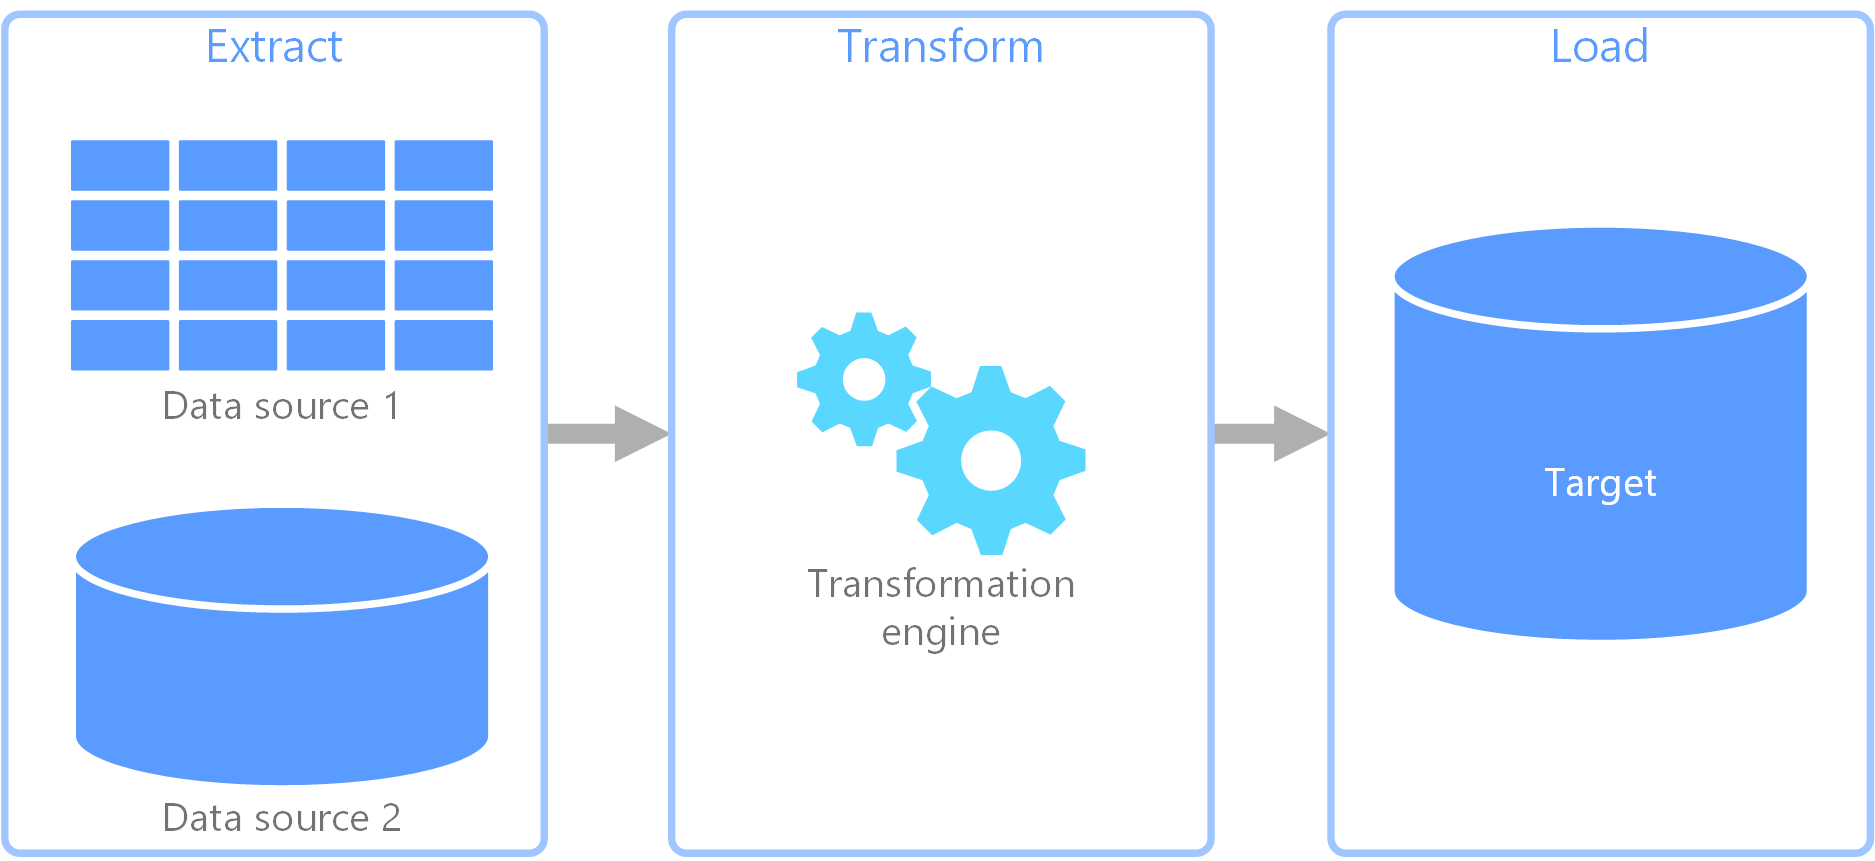
\includegraphics[width=0.80000\textwidth]{../images/etl.png}
\caption{etl\_process \label{figure_4}}
\end{figure}

Un processo di ETL si compone di tre parti:

La prima parte del processo di ETL è la fase di \textbf{Extract} ed
involve l'estrazione dei dati da più data sources come database
relazionali o non-relazionali, file JSON od XML ma anche risorse
``adhoc'' come, ad esempio, dei dati generati da programmi di web
analytics.

L'obiettivo di questa fase è estrarre tutti i dati necessari dalle
possibili sorgenti e prepararli alla fase di Transform.

Un importante problema legato a questa fase è il processo di
\textbf{validazione delle sorgenti dati}: con più sorgenti dati spesso
ci si ritrova a dover gestire più \emph{formati} non necessariamente
compatibili tra loro.\\
Per poter garantire alla fase di Transform dei dati comprensibili,
durante la fase di Extract vengono definite delle \emph{regole di
validazione} per filtrare i dati provenienti dalle varie sorgenti, un
esempio di regola di validazione è il controllo dei tipi di dati
presenti nella fonte.

\newpage

Nella fase di \textbf{Transform} una serie di regole e funzioni vengono
applicate ai dati generati dalla fase di Extract per prepararli alla
fase di Load nella data warehouse.

Il primo compito della fase di Transform è la \textbf{pulizia dei dati}:
spesso le varie fonti di dati, nonostante siano state validate, possono
presentare incongruenze tra loro come caratteri speciali legati
all'encoding della propria sorgente oppure formati dei dati diversi ma
compatibili (un esempio può essere la differneza di formattazione tra
date americane ed europee).\\
Per garantire un corretto funzionamento delle operazioni di
trasformazione è quindi necessario pulire i dati ed adattarli ad un
formato comune.

Il secondo compito della fase di Transform è la \textbf{trasformazione
dei dati} in nuovi dati richiesti dal business, esempi di trasformazioni
sono:

\begin{itemize}
\tightlist
\item
  Joining di tabelle da più sorgenti
\item
  Mapping e trasformazione di dati (esempio: ``Maschio'' in ``M'')
\item
  Aggregazione di dati
\item
  Generazione/calcolo di nuovi dati
\item
  Selezione di insiemi di dati
\item
  Validazione del nuovo formato di dati prodotto
\end{itemize}

Nella fase di \textbf{Load} l'insieme di dati generati dalla fase di
Transform vengono inseriti in un target, il quale potrebbe essere una
data warehouse ma anche più semplicemente un file in un formato utile.\\
Business diversi hanno necessità diverse, per questo l'implementazione
della fase di load può avere più modalità implementative, il punto
focale di questa fase è proprio stabilire la frequenza e le modalità di
aggiornamento dei dati presenti nel target.\\
Decidere la frequenza (giornaliera, mensile, ecc.) e le modalità
(sovrascrizione dei vecchi dati o meno) del target possono portare ad un
processo di ETL più o meno utile ad una azienda.

Per generare un buon target è buona norma definire uno schema
\emph{preciso e chiaro} della tipologia di dati a cui il target deve
aderire.\\
Come detto in precedenza un processo di ETL è utilizzato per aggregare
più fonti di informazioni comuni ad un processo aziendale, questo
suppone che le informazioni presenti nella data warehouse potrebbero
venire usate da più parti di una azienda, le quali potrebbero essere
abituate a particolari formati dei dati.\\
Senza definire uno schema dei dati chiaro e preciso, si correrebbe il
rischio di generare un insieme di dati inutilizzabile da determinati
reparti in quanto non conforme al formato di dati da loro conosciuto.

\newpage

\hypertarget{event-sourcing}{\subsection{4. Event
sourcing}\label{event-sourcing}}

\subsubsection{4.1. L'importanza dei dati e degli
eventi}\label{limportanza-dei-dati-e-degli-eventi}

Lo status quo delle moderne applicazioni web è basato sul utilizzo di
database per rappresentare le specifiche di dominio, spesso espresse da
un cliente e/o da un esperto del dominio esterno all'ambiente di
sviluppo.

Durante la fase di analisi dei requisiti (supponendo un modello di
sviluppo del software agile) cliente e team di sviluppo si confrontano,
cercando di trovare un linguaggio comune per definire la logica e
l'utilizzo del software richiesto; Una volta stabiliti i requisti, il
team di sviluppo generalmente inizia uno studio interno atto a produrre
un \textbf{modello dei dati} che verrà usato come base per definire lo
schema dei database utilizzati dal sistema.\\
Un cliente comune molto spesso non ha padronanza del concetto di `stato
di una applicazione', ma piuttosto si limita ad esporre i propri
requisiti descrivendo i possibili \textbf{eventi} che, traslati sul
modello di sviluppo incentrato su i database, portano il team di
sviluppo a ragionare sui possibili stati di un database in risposta a
questi eventi.

Lo stato di un database di una applicazione è strettamente legato
all'insieme degli eventi del dominio applicativo; L'unico modo per
modificare o interagire con questo database è tramite i comandi di
inserimento, cancellazione o lettura, tutti comandi che vengono eseguiti
solamente all'avvenire di un particolare evento.

Un database mantiene solo lo stato corrente di una applicazione; Non
esiste il concetto di cronologia del database a meno di utilizzare
soluzioni basate su \textbf{Change Data Capture} (CDC), generalmente
utilizzate per generare un transactional log contenente tutte le
operazioni eseguite sul suddetto database.\\
In questo modello database-driven, un evento genera un cambiamento su
una base di dati; Gli eventi e lo stato di un database sono però
concetti diversi e slegati tra loro, l'esecuzione di un evento a volte
può portare ad una asincronia tra l'esecuzione di un evento e lo stato
di un database, tanto più se questo database è utilizzato da tutti i
microservizi di una applicazione.

Una soluzione al problema di più microservizi che utilizzano lo stesso
database è di utilizzare delle views del database locali ad ogni
microservizio: ogni servizio lavorerà su una copia locale del database
ed un job esterno si occuperà di compattare le views e mantenere il
database aggiornato rispetto a tutti i cambiamenti.\\
Questa soluzione ha un enorme problema: supponiamo di notare un errore
sul database e di doverlo correggere, come possiamo decidere quale delle
views è ``più corretta'' delle altre? Per aiutarci nella ricerca
dell'errore potremmo utilizzare il transactional log di ogni views, ma
su database di grandezze importanti esaminare il log di ogni views che
lo compone potrebbe essere un problema complesso e dispendioso in
termini di tempo.

Event sourcing propone di risolvere questo genere di problemi
allontanandosi da una progettazione state-driven elevando gli eventi a
elementi chiavi del modello dei dati di una applicazione.

\subsubsection{4.2. Descrizione}\label{descrizione}

Event sourcing (ES) è un design pattern che si contrappone ad una
visione del mondo basata sullo stato di una applicazione fornendo come
alternativa l'uso degli eventi, ovvero delle azioni o accadimenti che
l'applicazione è in grado di riconoscere e gestire.

Durante l'analisi dei requisiti di una applicazione, spesso ci si trova
a confronto con esperti di un dominio applicativo che non hanno
particolare conoscenza delle tecnologie necessarie per implementare le
loro richieste, è compito del programmatore (o del team di
programmatore) analizzare le sue richieste e trasformarle in idee
gestibili.\\
In genere questi esperti spiegheranno al programmatore le loro necessità
illustrando il funzionamento del dominio utilizzando concetti molto più
vicini a degli \emph{eventi} piuttosto che \emph{sequenze di
richieste/risposte a/da un database}; Supponendo di dover sviluppare una
piattaforma di e-commerce, è molto più probabile che l'esperto di
dominio richieda di gestire eventi come ``aggiungere un oggetto al
carrello'' oppure ``comprare un oggetto'' piuttosto che ``creare dei
database per gestire carrello, stock oggetti rimamenti, oggetti
comprati''.

La struttura dati fondamentale alla base di ES è l'\textbf{event store},
una tipologia di database ottimizzata per la gestione di eventi.\\
In un event store, gli eventi vengono inseriti in fondo alla struttura
in ordine di avvenimento e non possono essere modificati o cancellati;
Nel caso venga pubblicato per errore un evento sbagliato o inesatto per
annularlo basterà pubblicare un evento contrario. Questo meccanismo
garantisce che la ripetizione della storia degli eventi \emph{porterà
sempre allo stesso stato, errore compreso}.

Un event store è comunemente implementato utilizzando un \textbf{log},
una sequenza di record append-only e totalmente ordinata in base al
tempo di scrittura del record.

\begin{figure}
\centering
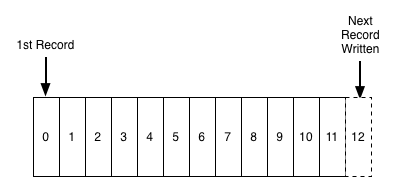
\includegraphics[width=0.68000\textwidth]{../images/log.png}
\caption{log\_data\_structure \label{figure_1}}
\end{figure}

I record sono inseriti in fondo al log e il processo di lettura è
eseguito partendo dall'inizio del log.

Generalmente in un processo di sviluppo basato su ES, si tende a
nominare gli eventi con il tempo passato per esplicitare il concetto che
un evento è un avvenimento passato, un esempio nome per un evento
potrebbe essere \texttt{item\_created} oppure \texttt{item\_bought}.

L'ordine di pubblicazione degli eventi è di estrema importanza in quanto
è ciò che permette al pattern di rappresentare correttamente lo stato di
una applicazione.

E' possibile vedere lo \textbf{stato corrente di una applicazione} come
una \textbf{sequenza di operazioni di modifica dello stato eseguite
partendo da uno stato iniziale}, questo implica che è possibile vedere
un \textbf{evento} come il \textbf{delta tra lo stato iniziale di una
applicazione e lo stato corrente dell'applicazione dopo l'esecuzione
dell'evento}.\\
La possibilità di trasformare lo stato corrente di una applicazione in
una funzione dello stato iniziale dell'applicazione e una sequenza di
eventi è il meccanismo che permette ad event sourcing di avere una
validità tecnica per la gestione dei dati di una applicazione.

\begin{figure}
\centering
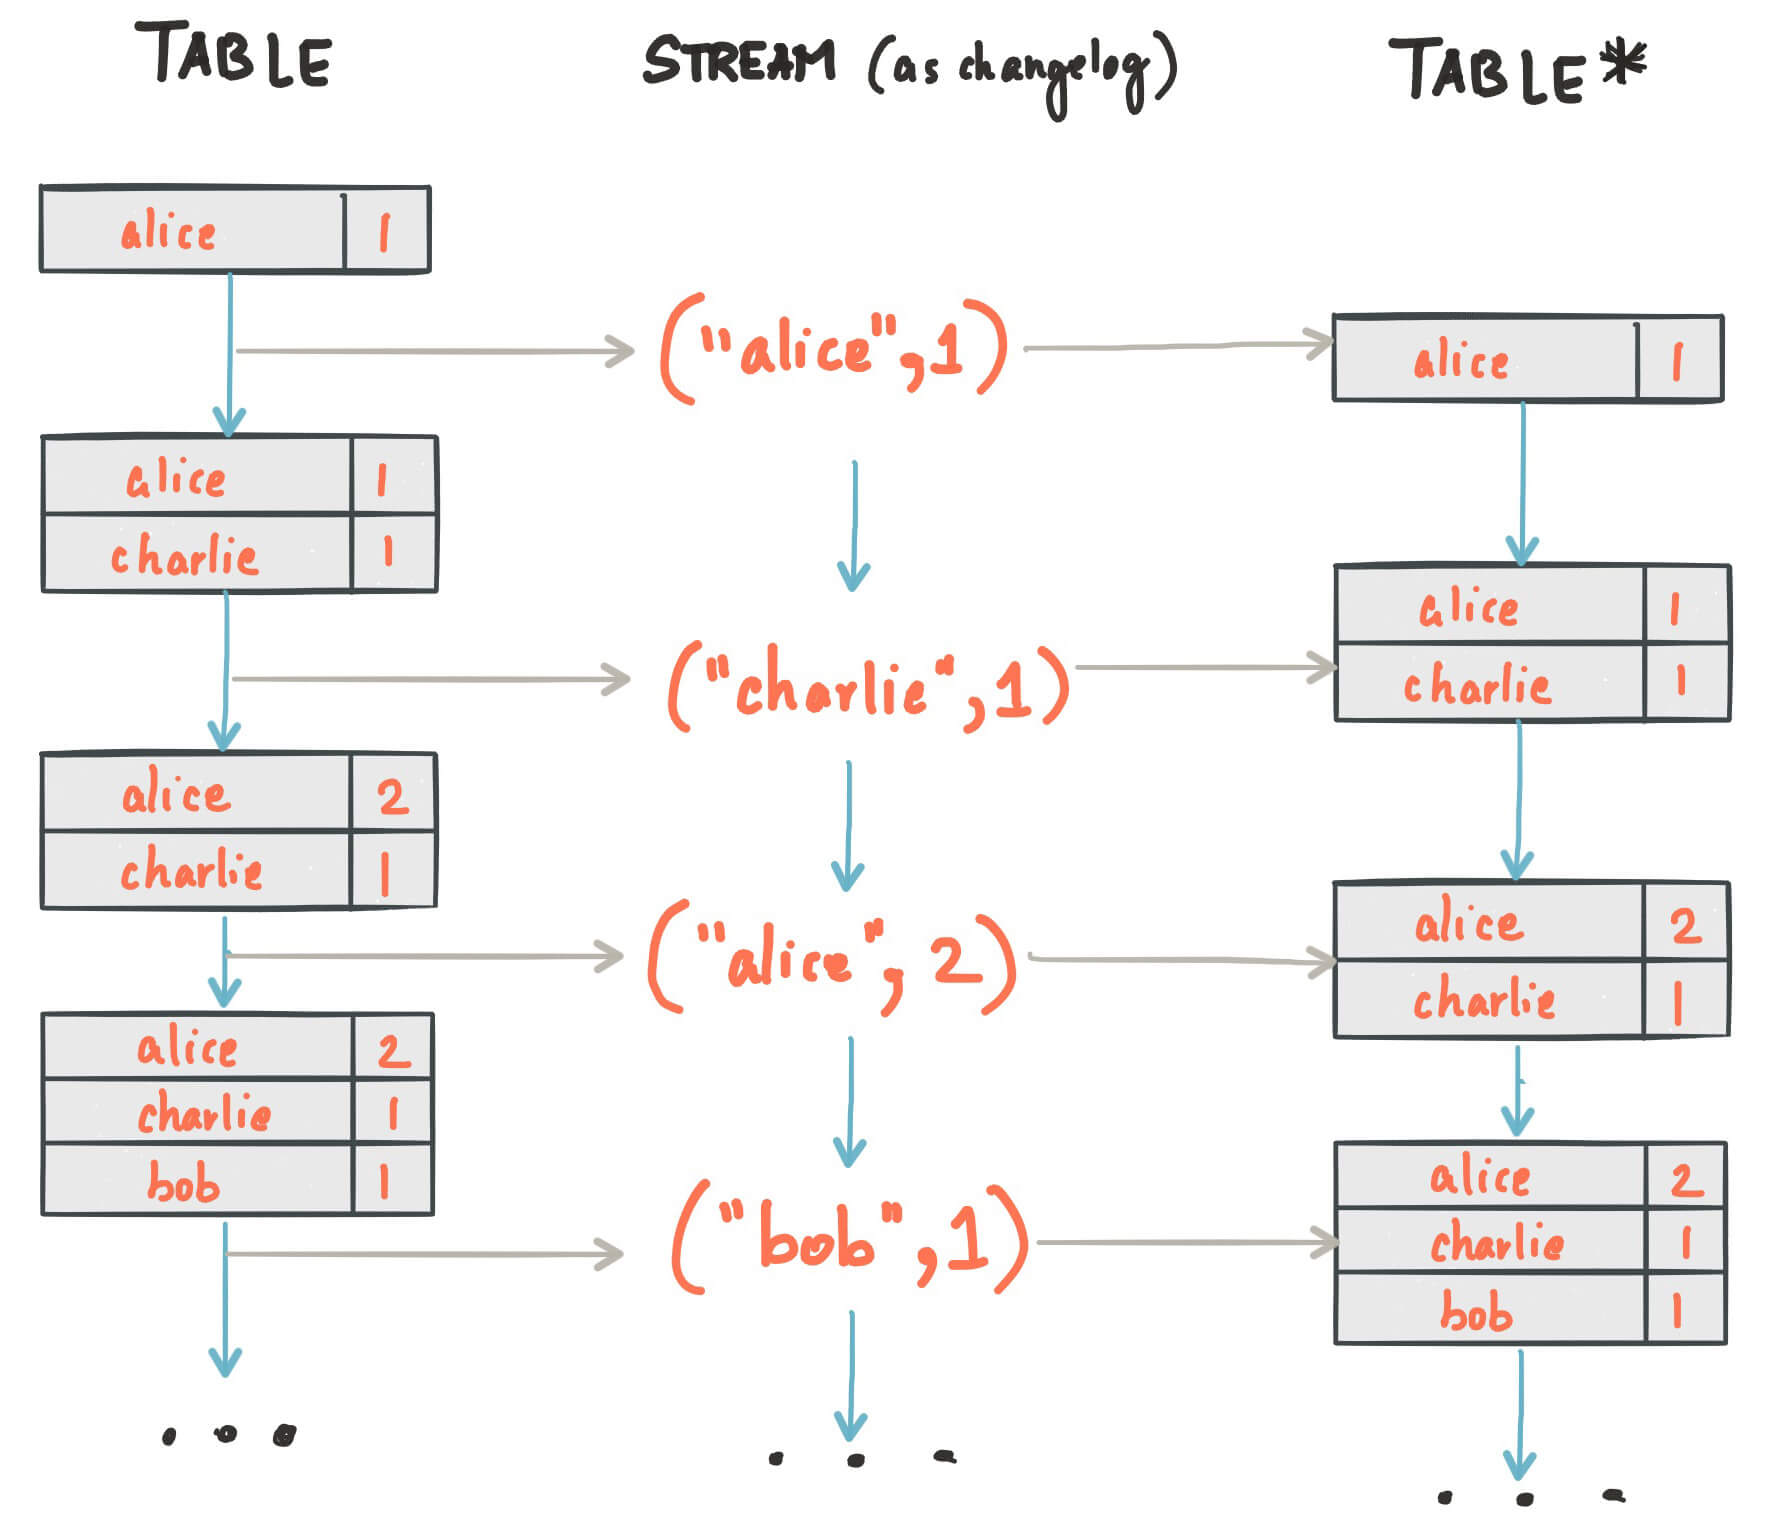
\includegraphics[width=0.80000\textwidth]{../images/streams-table-duality.jpg}
\caption{event\_log\_database\_duality \label{figure_2}}
\end{figure}

\newpage

\subsubsection{4.3. Vantaggi}\label{vantaggi}

Event sourcing è un pattern estremamente utile per tutti quegli use-case
dove è assolutamente necessario mantenere una storia dello sviluppo
dello stato dell'applicazione del tempo. Tipici esempi sono gli
strumenti di versioning del codice oppure la gestione di un storico
bancario.

La capacità dell'event store di essere sia una struttura dati
performante per la scrittura dei dati (è una semplice operazione di
scrittura in fondo ad una sequenza di complessità O(1)) che una
cronologia di tutti gli avvenimenti del sistema, permette una gestione
degli errori estremamente semplice.

In un qualsiasi database relazionale se durante il normale utilizzo
dell'applicazione avviene un errore logico che porta il database ad uno
stato non corretto, è sempre necessario un rollback dell'intero database
ad un data antecedente l'errore per poter sperare di correggiare
l'errore.\\
Tale processo è dispendioso in termini di tempo e non è di facile
esecuzione in quanto spesso il processo di backup di un database non
viene eseguito dopo ogni inserimento o update di un record; Per poter
correggere l'errore sarà quindi necessario calcolare partire dal backup
più recente e applicare nuovamente tutte le transformazioni del
database, meno l'errore.

L'analisi del motivo dell'errore può inoltre non essere di facile
realizzazione con un database relazionale a meno che non siano in uso i
meccanismi di CDC: senza una cronologia delle transazioni può essere
molto difficile risalire al motivo dell'errore.

Diversamente nel caso dell'utilizzo di Event Sourcing, la gestione e
l'analisi di un errore è estremamente semplice. Nel caso in cui
l'errore, che sarà sempre un evento, non ha generato un effetto
``domino'' sul sistema (ovvero l'errore non ha portato all'esecuzione di
uan catena di errori), una volta individuato è possibile pubblicare un
evento ``contrario'' alla causa dell'errore in modo tale da cancellare
l'apporto dell'errore sul sistema.\\
Nel caso contrario, ovvero il caso in cui l'errore ha generato una
sequenza di errori, per ottenere lo stato corretto del sistema basterà
ripetere l'esecuzione di tutti gli eventi del sistema escludendo quello
che ha generato l'errore sulla base di dati.

E' bene notare che con ES la gestione degli errori nello stato del
sistema è strettamente legata all'atomicità e definizione degli eventi
del sistema: una corretta (semplice) definizione degli eventi del
sistema porterà ad una cronologia del sistema più chiara e
comprensibile.

\newpage

\subsubsection{4.4. Svantaggi}\label{svantaggi}

Event sourcing potrebbe non essere utile per una applicazione che
richiede frequenti e continue query di richiesta sullo stato del
sistema.\\
Come descritto in precedenza, per ottenere lo stato corrente del sistema
è necessario eseguire tutti gli eventi pubblicati sull'event store
partendo da uno stato iniziale; Se la nostra applicazione richiede di
eseguire molte query di ricerca sullo stato corrente del database sarà
quindi necessario calcolare lo stato del sistema \emph{ogni volta che
viene eseguita una nuova richiesta} (un esempio di richiesta sullo stato
è la ricerca di tutti i record che presentano una particolare
caratteristica).

Le modalità per risolvere questo problema sono determinate dal dominio e
uso dell'applicazione che utlizza ES, ma generalmente per ovviare a
questa debolezza vengono realizzati degli snapshot dello stato
dell'applicazione da utilizzare per l'esecuzione delle query di ricerca.
La frequenza di generazione ed aggiornamento di questi snapshot è
strettamente legata al dominio applicativo dell'applicazione.

\newpage

\subsection{5. Apache Kafka e
l'ecosistema}\label{apache-kafka-e-lecosistema}

\emph{Publish/Subscribe} è un pattern architetturale utilizzato per la
comunicazione asincrona tra diversi processi od oggetti.

In questo schema mittenti e destinatari dialogano tra loro per mezzo di
un \emph{broker}, un processo incaricato, da una parte, di ricevere
messaggi da dei mittenti e dall'altra di consegnare gli stessi messaggi
a dei destinatari.

I destinatari non conoscono i mittenti, ed i mittenti non si interessano
di chi sono i destinatari: l'unico compito del mittente è quello di
pubblicare dei messaggi sul broker, starà poi al destinario il compito
di abbonarsi (dall'inglese \emph{subscribe}) al broker in modo da
ricevere tutti i nuovi messaggi.

Questo pattern viene spesso utilizzato quando ci si trova ad avere più
processi o servizi che generano delle metriche o dei dati, i quali sono
di vitale importanza per altrettanti servizi; Una soluzione alternativa
sarebbe creare dei canali dedicati tra produttori e consumatori ma
questo non permetterebbe alla struttura di supportare un numero sempre
più elevato di servizi od oggetti, ed in un mondo dove è sempre più
frequente l'utilizzo di microservizi e il logging di eventi e dati (Big
Data) porterebbe ad un debito tecnologico elevato e difficile da
correggere.

E' in questo contesto che nasce Apache Kafka, una \emph{streaming
platform} basata su un append-only log utilizzato da dei \emph{producer}
per pubblicare dei messaggi utilizzati da dei \emph{consumer}.\\
I messaggi pubblicati vengono persistiti nel tempo, sono leggibili
deterministicamente da qualsiasi consumer ed distributi all'interno del
sistema secondo particolari logiche in modo da garantire protezione da
crash e scalabità del sistema.

\newpage

\subsubsection{Messaggi}\label{messaggi}

L'unità dati fondamentali in Kafka è chiamata \emph{messaggio} o
\emph{record}.

Ogni messaggio è suddiviso in \emph{key} (opzionale) e \emph{value} e
possono essere di qualsiasi formato; Kafka non impone particolari
standard riguardo i formati dei dati utilizzabili all'interno del
sistema ma con lo scorrere del tempo \emph{Avro} è diventato lo standard
de facto.\\
Il campo \texttt{key}, quando definito, è un byte array utilizzato come
metadata per garantire un particolare ordinamento all'interno di un
\emph{topic}, un altro elemento fondamentale dell'architettura.

Nonostante Kafka sia una streaming platform, la scrittura e propagazione
dei messaggi all'interno della rete non avviene necessariamente per
messaggio, invece, piccoli gruppi di messaggi diretti verso la stesso
topic vengono raggruppati in \emph{batches}.\\
La gestione dei messaggi in batch nasce per motivi di efficienza per
bilanciare throughput e latenza: a fronte di una latenza più alta per la
consegna di un batch, vengono sprecate meno le risorse del sistema che
altrimenti si ritroverebbe costretto a gestire l'overhead di conoscegna
di un batch per ogni singolo messaggio.

\newpage

\subsubsection{Topic e partizioni}\label{topic-e-partizioni}

Un \emph{topic} è un elemento utilizzato in Kafka per categorizzare una
collezione di messaggi, e consiste in un unico stream di dati.

Un topic è suddiviso in \emph{partizioni}, append-only logs sui quali
vengono persisti i messaggi generati dai \emph{producers}.

\begin{figure}
\centering
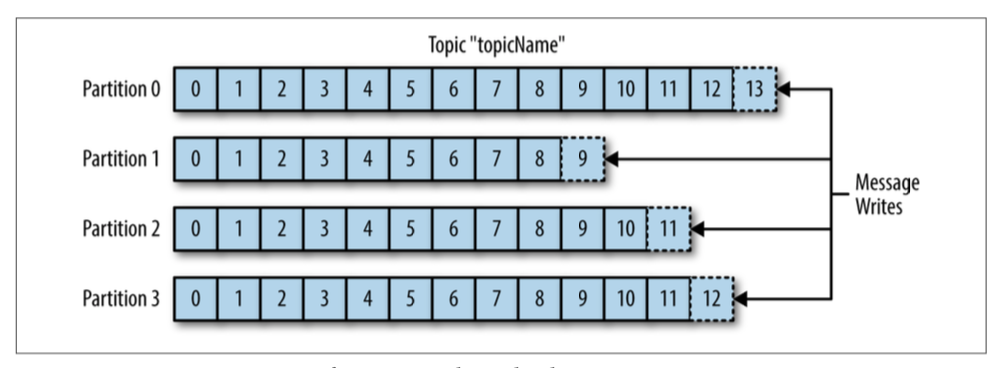
\includegraphics[width=0.90000\textwidth]{../images/topic-and-partitions.png}
\caption{Un topic suddiviso in più partizioni \label{figure_3}}
\end{figure}

I messaggi sono inseriti in una partizione da un producer nell'ordine in
cui sono stati inviati posizionandoli in fondo al log, non sono
modificabili o cancellabili e sono contradistinti da un \emph{offset},
un indice numerico che funziona da timestamp del messaggio. Un consumer
legge i messaggi di un topic partendo dalla testa (o da uno specifico
offset) del log proseguendo fino alla coda.

L'ordine di scrittura è garantito solo per ogni singola partizione: non
è detto che messaggi appartenenti al medesimo topic siano in ordine
cronologico se inseriti su partizioni diverse.

Per dare un esempio pratico di topic, supponiamo di utilizzare Kafka per
creare uno storage di eventi ricevuti dal front-end di una applicazione:
tipici eventi che vengono spesso loggati da un front-end possono essere
\emph{i link cliccati in una pagina}, \emph{quali pagine sono state
visualizzate in una sessione} oppure \emph{se è stato visualizzato un
particolare video embdeed}.\\
Per ogniuno di questi eventi verrà creato un singolo \texttt{topic} per
raggruppare tutte le notifiche e dati generati da uno di quei
particolari eventi a front-end: ad esempio avremo il topic
\texttt{views-video-embdeed} sul quale verranno registrati dei semplici
\texttt{yes} o \texttt{no} con magari l'aggiunta di un
\texttt{timestamp} (l'ora di visualizzazione), in questo modo il topic
ci permetterà di calcolare la frequenza di visualizzazione del video.

\newpage

\subsubsection{Producers e consumers}\label{producers-e-consumers}

L'architettura offerta da Kafka è utilizzata da due genere di client:
\emph{producers} oppure \emph{consumers}.

I \emph{producers} hanno il compito di creare messaggi indirizzati a
specifici topic (indipendentemente dal numero di partizioni da cui sono
formati).\\
Come illustrato in precedenza, un topic è formato da un numero variabile
di partizioni utilizzate come meccanismo di replica e gestione dei
messaggi; Alla creazione di un messaggio è possibile indicare al
producer su quale partizione andare a scrivere il record specificando
l'identificativo di una partizione specifica.

\begin{figure}
\centering
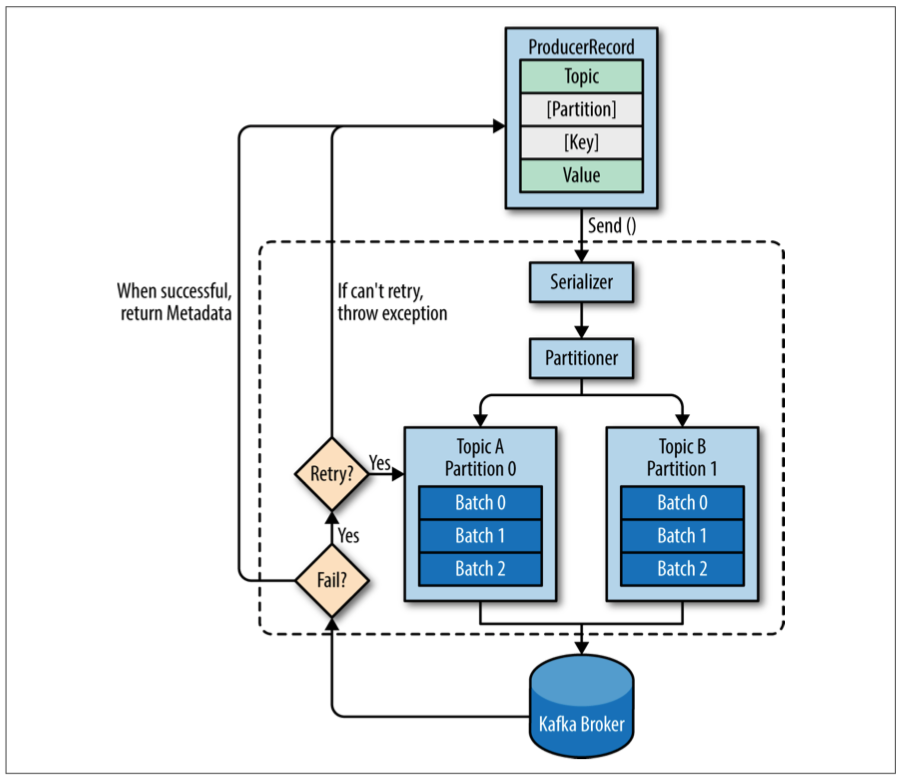
\includegraphics[width=0.90000\textwidth]{../images/producer-process.png}
\caption{Processo di pubblicazione di un messaggio \label{figure_3}}
\end{figure}

Il processo di pubblicazione di un messaggio inizia con la produzione di
un \texttt{ProducerRecord} il quale deve contenere il topic sul quale
vuole pubblicare il messaggio ad una value, ovvero il contenuto del
messaggio; Opzionalmente è possibile specificare una chiave o una
partizione specifica.\\
Nella maggior parte dei casi d'uso di Kafka, il producer non si pone mai
il problema di decidere su quale partizione andare a scrivere un
particolare messaggio ma piuttosto vengono utilizzati dei meccanismi di
load-balancing per spartire correttamente i messaggi su tutte le
partizioni disponibili presenti nel topic.\\
Tipici esempi di algoritmi di load-balancing sono il calcolo della
partizione in base ad una hash key derivata dall'offset del messaggio
oppure utilizzando un algoritmo round robin, se necessario è presente la
possibilità di specificare un \emph{partioneer} creato su misura al caso
d'uso.

Una volta creato il \texttt{ProducerRecord} il producer serializza
chiave e value del messaggio in \texttt{ByteArray} in modo da
effettivamente trasmetterli sulla rete. I dati sono quindi recapitati ad
un partitioner che andrà a deciderà su quale partizione pubblicare il
messaggio (solo nel caso in cui la partizione non era già stata
specificata nel record). Il record viene quindi aggiunto ad un batch di
record e il producer resta in attesa di avere abbastanza record (o
alternativamente, in attesa della scadenza di un timeout) prima di
inviare il batch di messaggi ad un broker.

Una volta che il broker riceve il batch di messaggi verranno effettuati
una serie di controlli per garantire la validità dei messaggi del batch
rispetto al topic su cui si sta cercando di pubblicare questi messaggi;
In caso positivo il broker invia al producer un \texttt{RecordMedatada}
con topic, partizione e offset dei messaggi dei pubblicati, altrimenti
ritornerà un errore. In caso di errore, il producer può provare a
rinviare il batch di messaggi.

I \emph{consumers} leggono i messaggi pubblicati sui topic ai quali si
sono iscritti.\\
I messaggi possono essere letti partendo dalla testa (o inizio) del
topic oppure uno specifico \emph{offset} fino ad arrivare alla coda (o
fine).\\
Un \emph{offset} è un identicativo numerico corrispondente ad una chiave
per uno specifico messaggio del topic ed è compito del consumer di tener
traccia degli offset di tutti i messaggi che lui stesso ha già letto.\\
L'offset di un messaggio è \emph{specifico ad una specifica
\textbf{partizione}}.\\
La capacità di mantenere in memoria gli offset dei messaggi già letti
garantisce al consumer la capacità di fermare, ed in un secondo momento
reiniziare, il processo di lettura di un topic.

\begin{figure}
\centering
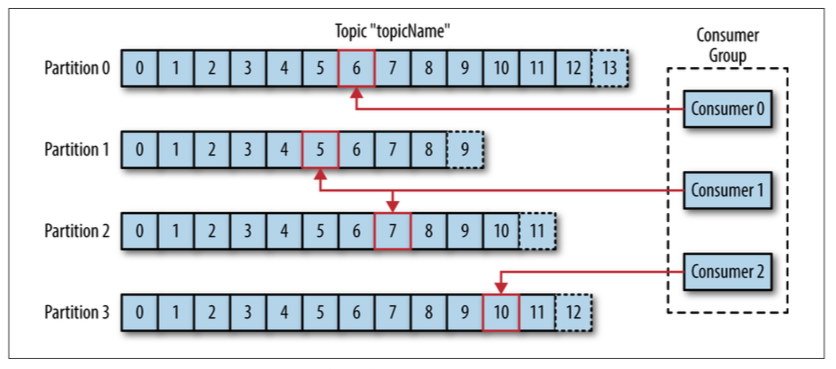
\includegraphics[width=0.90000\textwidth]{../images/topic-and-consumers.png}
\caption{Esempio di un topic letto da un gruppo di consumers
\label{figure_3}}
\end{figure}

\newpage

I consumers lavorano in \emph{gruppi di consumers}: uno o più consumer
lavorano per leggere un intero topic, con la proprietà che
\emph{consumers diversi non possono leggere dalla stessa partizione}.

Questa struttura porta ad un alto throughput in lettura di un topic
permettendo uno sviluppo orizzontale del numero di consumers necessari
per leggere un numero elevato di messaggi per partizione. Nel caso di un
crash di uno dei consumer un consumer group è dotato di un meccanismo di
load balancing che permetterà ad un altro consumer del gruppo di
continuare a leggere i messaggi della partizione che stava venendo
consumata.

\subsubsection{Brokers e clusters}\label{brokers-e-clusters}

Un \emph{broker} è un server Kafka con svariati compiti quali ricevere,
indicizzare e salvare i messaggi inviati dai producers ed inviare i
messaggi richiesti dai consumers; Un singolo broker è capace di gestire
miglialia di partizioni e millioni di messaggi al secondo.

I broker sono stati creati per lavorare in \emph{clusters} ovvero gruppi
di brokers ordinanti secondo una particolare gerarchia.

\begin{figure}
\centering
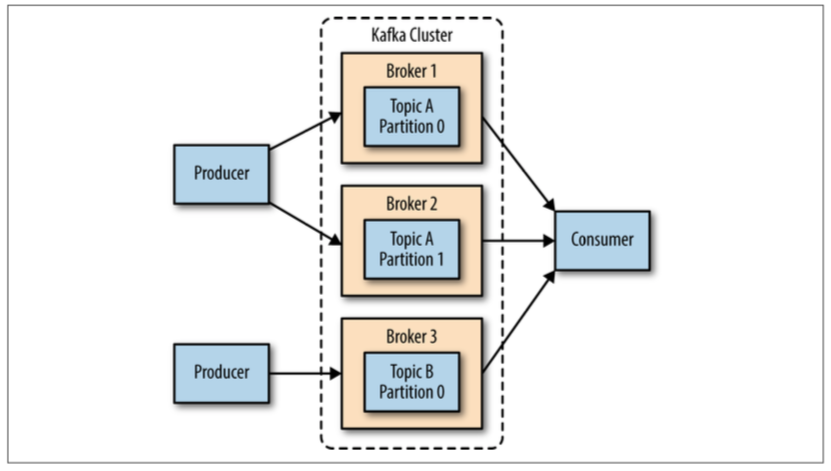
\includegraphics[width=0.90000\textwidth]{../images/kafka-cluster.png}
\caption{Esempio di cluster \label{figure_5}}
\end{figure}

A capo di un cluster troviamo un broker \emph{leader} al quale tutti gli
altri broker del cluster devono far riferimento per permette ai
meccanismi di replicazioni dei messaggi di funzionare correttamente: una
partizione può essere assegnata a più broker, questo permette al cluster
di avere un meccanismo per la gestione dei fallimenti dei brokers. In
ogni cluster un particolare broker viene eletto a \emph{controller},
ovvero un broker con l'incarico di gestire la suddivisione di partizioni
sull'intero cluster e di monitorare il cluster.

\begin{figure}
\centering
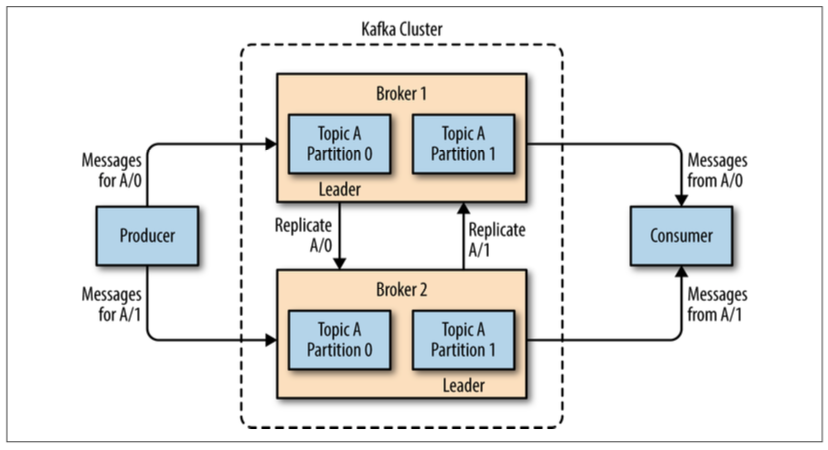
\includegraphics[width=0.90000\textwidth]{../images/partition-replica.png}
\caption{Gestione delle repliche \label{figure_5}}
\end{figure}

\newpage

Una funzionalità importante di Kafka è la possibilità di utilizzare i
topic come database di messaggi persistenti.\\
I messaggi vengono tenuti in memoria per un particolare periodo di tempo
oppure in base allo spazio di memoria di occupato, entrambe le opzioni
sono configurabili alla creazione di un broker, vi è poi la possibilità
di abilitare la \emph{log compaction} ovvero un meccanismo che permette
a Kafka di mantenere in memoria \emph{solo gli ultimi messaggi
indicizzati su un indicativo specifico}.

\newpage

\subsubsection{Schema}\label{schema}

Nonostante i messaggi in Kafka non siano altro che degli array di byte è
fortemente consigliato l'uso di \emph{schema} per la gestione e l'uso
della struttura dei record.

Lo \emph{schema} è la struttura o organizzazione logicati dei dati
contenuti in un topic e nel caso specifico di Kafka, la scelta dei
formati disponibili ricade spesso su di un singolo formato: Apache Avro.
Esistono altre scelte possibili come Javascript Object Notation (JSON)
oppure Extensible Markup Language (XML), ma Avro offre una serie di
vantaggi rispetto a questo genere di schemi oltre ad avere alcune
implementazioni ad-hoc in Kafka. Avro è diventato nel tempo lo standard
per gli schema nelle applicazioni basate su Kafka, gli stessi
sviluppatori di Kafka ne promuovono l'uso citando una serie di motivi:

\begin{itemize}
\tightlist
\item
  Avro è mappabile su JSON
\item
  Al contrario di JSON, è possibile scindere lo schema dei dati dalla
  definizione dell'oggetto/record
\item
  E' un linguaggio maturo con un importante supporto dalla community;
  Esistono molte librerie che permettono di creare automaticamente
  oggetti Java o case classes in Scala partendo da uno schema Avro
\end{itemize}

Apache Avro è un formato per la serializzazione di dati, ogni messaggio
Avro si divide in due parti: i \emph{dati} e lo \emph{schema dei dati}.

Un esempio di \textbf{schema dei dati} di un record con cinque campi:
\small

\begin{verbatim}
{
  "type": "record",
  "doc":"This event records the sale of a product",
  "name": "ProductSaleEvent",
  "fields" : [
    {"name":"time", "type":"long", "doc":"The time of the purchase"},
    {"name":"customer_id", "type":"long", "doc":"The customer"},
    {"name":"product_id", "type":"long", "doc":"The product"},
    {"name":"quantity", "type":"int"},
    {"name":"payment",
     "type":{"type":"enum",
         "name":"payment_types",
             "symbols":["cash","mastercard","visa"]},
     "doc":"The method of payment"}
  ]
}
\end{verbatim}

\normalsize
\newpage
Ed un generico record di \textbf{dati} definito in base allo schema:

\small

\begin{verbatim}
{  
  "time": 1424849130111,     
  "customer_id": 1234,  
  "product_id": 5678,  
  "quantity":3,  
  "payment_type": "mastercard"  
}
\end{verbatim}

\normalsize

In Kafka ogni topic posside un particolare schema Avro im modo da :

\begin{itemize}
\tightlist
\item
  definire la struttura dei messaggi pubblicabili nel topic
\item
  permettere a producers e consumers di conoscere quali sono i campi dei
  messaggi del topic e qual'è il loro tipo
\item
  documentare la tipologia dei messaggi pubblicati nel topic
\item
  evitare la presenza di dati corrotti nel topic
\end{itemize}

Questo genere di meccanismo per la gestione dei dati diventa di assoluta
importanza all'aumentare delle applicazioni che dipendono dall'utilizzo
dei dati prodotti e gestiti da una piattaforma Kafka, evitando problemi
``effetto Domino'' dove un singolo errore in un messaggio potrebbe
portare a corrompere un consumer o applicazioni terze che utilizzano i
dati forniti dal consumer.

Un formato dei dati consistente come Avro permette di \emph{disacoppiare
i formati utilizzati per la lettura e la scrittura dei messaggi}, ovvero
viene data la possibilità alle applicazioni che si iscrivono ad un
particolare topic di poter utilizzare un nuovo schema di dati
compatibile con un vecchio formato, senza dover aggiornare tutte le
applicazioni che utilizzano ancora il vecchio formato.

Supponiamo ad esempio di utilizzare un formato del tipo seguente per
gestire le informazioni riguardando agli acquirenti di un particolare
servizio/piattaforma:

\small 

\begin{verbatim}
{
    "namespace": "customerManagement.avro",
    "type": "record",
    "name": "Customer",
    "fields": [
         {"name": "id", "type": "int"},
         {"name": "name",  "type": "string"},
         {"name": "faxNumber", "type": ["null", "string"], "default": "null"}
    ] 
}
\end{verbatim}

\normalsize

Una applicazione che vuole utilizzare lo stream di dati di questo topic
avrà probabilmente dei metodi come \texttt{getId()}, \texttt{getName()}
e \texttt{getFaxNumber()} per leggere i dati del topic; Di nota è il
tipo del campo \texttt{faxNumber} il quale è esplicitamente possibile
che sia \texttt{null}, ovvero è lecito aspettarsi che l'applicazione che
utilizza questi dati non si romperà nel caso in cui il fax non sia
presente nel messaggio.

Supponiamo di aver utilizzato lo schema precedente per genere una
importante mole di dati in un topic ma di voler migrare il nostro schema
ad un nuovo formato che permetta agli utenti di specificare la loro
\texttt{email} piuttosto che il loro fax.

\small

\begin{verbatim}
{
    "namespace": "customerManagement.avro",
    "type": "record",
    "name": "Customer",
    "fields": [
         {"name": "id", "type": "int"},
         {"name": "name",  "type": "string"},
         {"name": "email", "type": ["null", "string"], "default": "null"}
    ] 
}
\end{verbatim}

\normalsize

Ancora una volta l'applicazione che utilizza questo schema avrà dei
metodi \texttt{getId()}, \texttt{getName()} ma invece di
\texttt{getFaxNumber()} avrà \texttt{getEmail()}; Dopo l'aggiornamento
dello schema, i vecchi messaggi presenti nel topic conterranno il campo
\texttt{faxNumber} mentre i nuovi messaggi avranno il campo
\texttt{email}.

Dato che il tipo dei campi \texttt{faxNumber} e \texttt{email} può
essere sia \texttt{string} che \texttt{null}, nessuna delle tue
tipologie di applicazioni potrà fallire: la vecchia tipologia di
applicazioni semplicemente registrerà i nuovi messaggi come utenti senza
un numero di fax, mentre le nuove applicazioni vedranno i vecchi
messaggi del topic come utenti senza una email.

Questo genere di \emph{evoluzione} dello schema dei dati di un topic è
il motivo centrale dietro all'uso della tecnologia: garantire la
robustezza dei dati senza compromettere la leggibilità dello schema o il
funzionamento di applicazioni che utilizzano lo stesso topic.\\
L'evoluzione dello schema è permessa solo secondo determinate regole di
compatibilità la cui definizione esula dal contesto di questo tesi ma
che possono essere visionate nella
\href{https://avro.apache.org/docs/1.7.7/spec.html\#Schema+Resolution}{documentazione
di Apache Avro}.

\newpage

\subsubsection{Schema Registry}\label{schema-registry}

Uno dei vantaggi di Avro rispetto a JSON è la possibilità di non dover
inserire lo schema dei dati ``completo'' in ogni record permettendo di
pubblicare su un topic dei messaggi meno pesanti rispetto a JSON ed è
proprio per sfruttare questo vantaggio che nasce lo \emph{Schema
Registry}.\\
Uno \emph{schema registry} è un servizio di gestione degli schema Avro
utilizzato da Kafka per servire ed evolvere i metadati di un topic; E'
utilizzato dai producers nella fase di scrittura (serializzazione di un
messaggio). dai consumer nella fase di lettura (deserializzazione di un
messaggio) ed impone delle regole di forma a tutti i client che
intendono utilizzare un topic specificato con formato dati Avro.

\begin{figure}
\centering
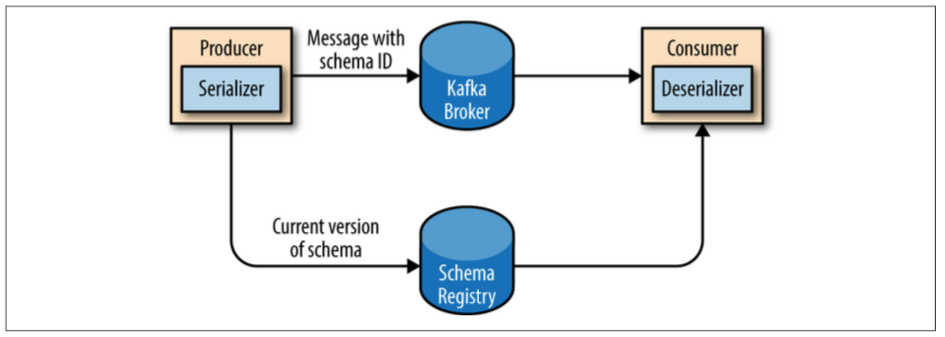
\includegraphics[width=0.90000\textwidth]{../images/schema-registry.png}
\caption{Serializzazione e deserializzazione con schema registry
\label{figure_5}}
\end{figure}

Supponiamo di avere uno schema registry e di voler produrre dei messaggi
su di un topic:

\begin{enumerate}
\def\labelenumi{\arabic{enumi}.}
\tightlist
\item
  Il producer interrogherà il registry per sapere se esiste già uno
  schema dei dati per un particolare topic inviando la propria copia
  dello schema, in caso contrario sarà lui stesso a pubblicarlo nel
  registry.
\item
  Lo schema registry verifica se lo schema ricevuto dal producer è
  uguale o una evoluzione compatibile dello schema già presente, in caso
  negativo verrà alzata un eccezzione e vietata la scrittura al
  producer.
\item
  Se lo schema proposto dal producer è valido, nel record Avro verrà
  inserito un riferimento allo schema del topic.
\end{enumerate}

L'utilizzo dello schema registry da parte di un consumer è speculare a
quello di un producer.

\newpage

\begin{quote}
Come collegare event sourcing e kafka =\textgreater{} perchè kafka è una
buona piattaforma per event sourcing
\end{quote}

\subsubsection{3.2 Kafka Connect}\label{kafka-connect}

\begin{quote}
Schema
\end{quote}

\begin{quote}
Source connectors
\end{quote}

\begin{quote}
Sink connectors
\end{quote}

\begin{quote}
Community involment
\end{quote}

\subsubsection{3.3 Kafka Streams}\label{kafka-streams}

\begin{quote}
cos'è streams
\end{quote}

\begin{quote}
KSQL/LSQL
\end{quote}

\subsection{8. Esempi di utilizzo di
Kafka}\label{esempi-di-utilizzo-di-kafka}

\newpage

\subsection{9. Bibliografia}\label{bibliografia}

https://engineering.linkedin.com/distributed-systems/log-what-every-software-engineer-should-know-about-real-time-datas-unifying
https://www.confluent.io/blog/stream-data-platform-1/
https://martinfowler.com/eaaDev/EventSourcing.html\\
https://en.wikipedia.org/wiki/Event\_store\\
https://www.confluent.io/blog/data-dichotomy-rethinking-the-way-we-treat-data-and-services/\\
https://www.confluent.io/blog/build-services-backbone-events/\\
https://www.confluent.io/blog/apache-kafka-for-service-architectures/\\
https://www.confluent.io/blog/messaging-single-source-truth/\\
https://www.confluent.io/blog/building-a-microservices-ecosystem-with-kafka-streams-and-ksql/\\
https://content.pivotal.io/blog/understanding-when-to-use-rabbitmq-or-apache-kafka\\
https://qconsf.com/sf2016/system/files/keynotes-slides/etl\_is\_dead\_long-live\_streams.pdf
\textless{}= https://www.youtube.com/watch?v=I32hmY4diFY

\end{document}
